\documentclass[11pt,a4paper]{article}
\usepackage[margin=2.2cm]{geometry}
\usepackage[T1]{fontenc}
\usepackage[utf8]{inputenc}
\usepackage{mathptmx}
\usepackage{microtype}
\usepackage{amsmath}
\usepackage{booktabs}
\usepackage{tabularx}
\usepackage{graphicx}
\usepackage{float}
\usepackage[font=small,labelfont=bf]{caption}
\usepackage{xcolor}
\usepackage{enumitem}
\usepackage[colorlinks=true,linkcolor=blue!50!black,urlcolor=blue!50!black,citecolor=blue!50!black]{hyperref}

\setlist{itemsep=1pt,topsep=3pt}
\setlength{\parskip}{3pt}
\emergencystretch=3em
\newcommand{\todo}[1]{\textcolor{red!75!black}{\textbf{[to do: #1]}}}
\newcommand{\code}[1]{\texttt{#1}}

\title{\vspace{-1.2cm}Auditing an income-prediction model for sex bias\\[2pt]
\large Supervised Learning \& Model Engineering (MSA-DATB09-04) --- Project report (draft)}
\author{Manel Rahali, Soumaya Atoui, Hadiqa Javaid\\[2pt]
\small Albert School, Fall 2026\\
\small Repository: \url{https://github.com/mrahali-cell/Supervised-Learning-Model-Engineering}}
\date{\vspace{-0.6cm}}

\begin{document}
\sloppy
\maketitle

\begin{center}
\fbox{\parbox{0.92\textwidth}{\centering\textbf{Dataset: Option 1 --- Adult / Census Income}\\
\code{fetch\_openml(name="adult", version=2)}, 48{,}842 people, 15 columns, 1994 US Census \cite{kohavi1996}.}}
\end{center}

\begin{abstract}
\noindent A company sells models that predict whether a person earns more than \$50K a year; its clients use the predictions for decisions such as audits. We perform the \emph{model-audit step}: build the best honest model the data allows, then measure how unequally it treats women and men, reduce part of that gap and show what it costs. This draft covers the first stages: problem framing, exploratory analysis, preprocessing and feature engineering, class imbalance, the model progression, and the tuning of logistic regression and the random forest. With six legitimate inputs, logistic regression, a random forest and LightGBM (default settings) reach the same level (about 0.71 PR-AUC, 0.89 ROC-AUC). For the random forest, validation curves show that limiting tree growth fixes its overfitting, and a search space built from these curves (tuning v2) keeps the ranking of the first tuning while restoring trustworthy probabilities (Brier 0.110 instead of 0.136). The EDA shows that the inputs are proxies for sex, which the later stages (calibration, explainability, fairness audit, test-set evaluation) will examine.
\end{abstract}

% ---------------------------------------------------------------
\section{Problem framing and evaluation protocol}

\paragraph{Use case.} If an income model treats some groups worse than others, the audit decisions built on it become unfair, and its clients face sanctions, legal action and financial loss. Our deliverable is the evidence an auditor needs: how biased the model is by sex, one mitigation, and what it costs. The research question is \emph{how biased by sex is a model that predicts income $>$ \$50K without ever seeing sex?} Our hypothesis is that it rebuilds the gender gap through proxies: marital status, occupation and hours worked.

\paragraph{Target and metrics.} The target \code{high\_income} = 1 if income $>$ \$50K (23.9\% of people). In an audit neither error dominates, so we chose the orientation that makes the metrics informative: the rare class as positive (Session~6). Accuracy is uninformative (always answering ``no'' scores 76\%), and ROC-AUC rewards the many correct rejections of low earners. We therefore rank models with \textbf{PR-AUC}, whose floor is the prevalence (0.239), report ROC-AUC beside it, and judge the probabilities with the \textbf{Brier score}. With the first orientation (low income = 1) the PR-AUC floor was 0.76 and every model scored about 0.96, which hid the differences.

\paragraph{Fairness definition, fixed before any result.} Primary: \textbf{equalized odds} (equal true- and false-positive rates for women and men) \cite{hardt2016}, because for a general-purpose model both kinds of error can harm someone. Legal screen: the \textbf{four-fifths rule} on selection rates. Demographic parity and predictive parity will also be reported (Section~\ref{sec:fair}).

\paragraph{Honest protocol.} After fixed cleaning rules, the data is split once into a development set (80\%, 39{,}032 people) and a test set (20\%, 9{,}758 people), stratified on the target (23.94\% high earners in both) with \code{random\_state=42}. All model choices use 5-fold stratified cross-validation on the development set; the test set stays locked until the final evaluation. Anything that learns from the data (imputation, scaling, encoding) lives inside the Pipeline and is re-fitted in every fold (Session~5). Table~\ref{tab:steps} maps the project to the course and the code.

\begin{table}[H]
\centering\small
\begin{tabularx}{\textwidth}{@{}c>{\raggedright}p{5.0cm}>{\raggedright}Xc>{\raggedright\arraybackslash}p{2.7cm}@{}}
\toprule
\# & Step & Where in the code & Req. & Status \\
\midrule
1--3 & Framing, EDA, cleaning, stratified split & \code{notebooks/01\_eda.ipynb}, \code{src/data.py} & 1 & done \\
4 & Feature engineering + preprocessing in one Pipeline & \code{src/pipeline.py} & 2, 5 & done \\
5 & Baseline progression: Dummy $\to$ LR $\to$ RF $\to$ LightGBM & \code{tuning/baseline.py} & 3, 4 & done \\
6--7 & Diagnosis (validation curves), Optuna tuning, MLflow & \code{tuning/random\_forest.py}, \code{tuning/tune.py} & 6, 7 & LR, RF done; LightGBM in progress \\
8 & Calibration & \code{src/evaluate.py} & 9 & to do on the final model \\
9 & Explainability (SHAP) & & 8 & to do \\
10 & Fairness audit and mitigation & \code{src/fairness.py} & 10 & to do on the final model \\
11 & Test set, once: final metrics, fairness before / after & & 9, 10 & to do \\
\bottomrule
\end{tabularx}
\caption{The project in 11 steps. Scripts run; notebooks only explain results; \code{docs/findings\_log.md} records every finding with its numbers.}
\label{tab:steps}
\end{table}

% ---------------------------------------------------------------
\section{Data and exploratory analysis}

\paragraph{Integrity.} Missing values affect three columns: \code{workclass} (5.73\%), \code{occupation} (5.75\%), \code{native-country} (1.75\%). They are not random: all 2{,}799 people missing \code{workclass} also miss \code{occupation}; the 10 extra missing occupations belong to people who never worked, for whom occupation is \emph{not applicable} (set to ``Never-worked''). Other missing values become an explicit ``Unknown'' category inside the Pipeline, which keeps the information that the value was missing. We removed 52 exact duplicates (0.11\%) so the same record cannot sit on both sides of the split. Extreme values are census caps (244 capital gains at 99{,}999; 137 people at 99 hours; 55 at age 90) and were kept; the IQR rule is unusable when 91.7\% of capital gains are zero. Categories with a few dozen people were merged by meaning and income rate: \emph{Without-pay} (21) and \emph{Never-worked} (10) into \emph{No-pay}, 37 \emph{Married-AF-spouse} into \emph{Married-civ-spouse}, 15 \emph{Armed-Forces} into \emph{Protective-serv}; \code{native-country} was grouped into United States / Mexico / Other. These fixed rules learn nothing from the data and are safe before the split.

\paragraph{Leakage audit.} For each column we asked whether it would be known at prediction time (Session~1). Capital gains fail: 98.4\% of people with a gain $\geq$ \$10{,}000 earn more than \$50K, and all 244 at the cap do; the variable is probably derived from income and is not collected by a short questionnaire. We dropped \code{capital-gain} and \code{capital-loss}. This is why our scores (about 0.89 ROC-AUC) must not be compared with published ones (0.92--0.93), which use them \cite{chakrabarty2018}.

\paragraph{Columns kept out.} \code{education} duplicates \code{education-num}; \code{fnlwgt} is a sampling weight, not a trait (medians 178{,}811 vs 176{,}729 by class); \code{relationship} reveals sex (all 19{,}716 Husbands and 2{,}331 Wives are married). \code{sex}, \code{race} and \code{native-country} are protected characteristics, kept only for the audit. Six inputs remain: \code{age}, \code{workclass}, \code{education-num}, \code{marital-status}, \code{occupation}, \code{hours-per-week}. The strongest signals are marital status (44.6\% of married people earn more than \$50K vs 4.5--10.1\% for the other statuses), occupation, education (15.9\% at level 9, 41.3\% at 13, 74.0\% at 15), work class and age.

\paragraph{Where the gender gap lives.} 30.4\% of men vs 10.9\% of women earn more than \$50K. Figure~\ref{fig:gap} shows that among married people the rates are equal (44.8\% vs 44.6\%), but 60.9\% of men are married vs 15.3\% of women, and gaps remain within education and hours groups. Occupations differ too (25.3\% of women in administrative jobs vs 5.9\% of men; 2.2\% vs 18.6\% in craft and repair), and women work 36.4 hours on average vs 42.4 for men. Leaving \code{sex} out therefore does not make a model blind to it: its inputs are proxies (``fairness through unawareness'' fails, Session~9). These are descriptive associations, not causes. The split keeps enough people per sex to audit (356 high-earning women in the test set), but two race groups have fewer than 100 people in the test set and can only be described.

\begin{figure}[H]
\centering
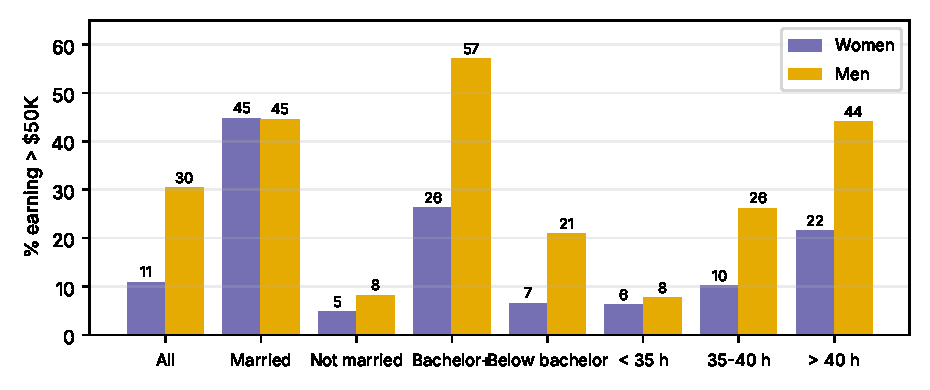
\includegraphics[width=0.78\textwidth]{figures/eda_gap.pdf}
\caption{Share earning $>$ \$50K, women vs men, overall and within groups (EDA). Married women and men have the same rate; the overall gap comes largely from who is married, plus gaps within education and hours groups.}
\label{fig:gap}
\end{figure}

% ---------------------------------------------------------------
\section{Feature engineering and the Pipeline}

Each engineered feature is a fixed rule justified by an EDA pattern (share earning $\leq$ \$50K in the development set):
\begin{itemize}
\item \code{is\_married}: married 55.5\% vs everyone else 93.6\%;
\item \code{has\_degree} (\code{education-num} $\geq$ 13, a bachelor's degree or more): 52.0\% vs 83.9\%;
\item \code{part\_time} ($<$ 35 h) and \code{overtime} ($>$ 40 h): about 93\% below 35 h, 78.7\% at 40 h, 56--65\% above 40 h. Both medians are 40 h, which had hidden this signal in the first EDA;
\item \code{age\_squared}: income rises with age, then falls (98.9\% at 24 or younger, 60.6\% at 45--54, 79.6\% at 65+), a U-shape a linear model cannot draw from \code{age} alone.
\end{itemize}
The Pipeline (\code{build\_pipeline(model)}) chains a \code{FunctionTransformer} that adds these features, a \code{ColumnTransformer} and the model. Numbers are imputed with the training median (the most neutral choice) and standardized; categories get ``Unknown'' then one-hot encoding with \code{handle\_unknown="ignore"}, so a category absent from a training fold does not crash; the binary features pass through. Six inputs become 37 columns (32 without the engineered features). One-hot encoding avoids inventing an order between categories; scaling matters for the regularized logistic regression and changes nothing for trees. The features lift logistic regression from 0.688 to 0.708 PR-AUC; the tree models find the same patterns by themselves (Table~\ref{tab:models}).

% ---------------------------------------------------------------
\section{Class imbalance}

The positive class is 23.9\% of people. We tested class weighting as the course suggests, as a hyperparameter: \code{class\_weight="balanced"} for logistic regression and the random forest, \code{scale\_pos\_weight} for LightGBM. Weighting never improved the ranking and always degraded the probabilities (Table~\ref{tab:imbalance}). Session~6 notes that weights help when a model underfits the rare class; ours do not. We therefore do not re-weight: the imbalance will be handled by the \textbf{decision threshold}, chosen at the decision stage, which leaves the probabilities intact \todo{threshold choice, with the fairness audit}. We did not use SMOTE: half of our inputs are categorical, a case where interpolating between people is undefined. In the code, weights are part of the Optuna search spaces (\code{tuning/tune.py}).

\begin{table}[H]
\centering\small
\begin{tabular}{@{}lccc@{}}
\toprule
Model (5-fold CV, development set) & PR-AUC & ROC-AUC & Brier \\
\midrule
Logistic regression, no weights (base features) & 0.688 & 0.883 & 0.114 \\
Logistic regression, balanced weights (base features) & 0.684 & 0.883 & 0.143 \\
LightGBM defaults, no weights & 0.716 & 0.892 & 0.110 \\
LightGBM defaults, balanced weights & 0.716 & 0.892 & 0.137 \\
Random forest (200 trees, sklearn defaults), no weights & 0.642 & 0.859 & 0.130 \\
Random forest (200 trees, sklearn defaults), balanced weights & 0.628 & 0.859 & 0.145 \\
\bottomrule
\end{tabular}
\caption{Class weights leave the ranking unchanged or worse and degrade the probabilities (higher Brier score).}
\label{tab:imbalance}
\end{table}

% ---------------------------------------------------------------
\section{Modelling progression}

Table~\ref{tab:models} compares the course progression on the same folds and metrics, all with default settings. The fold-to-fold standard deviation of PR-AUC is about 0.013, so smaller differences are not real.

\begin{table}[H]
\centering\small
\begin{tabular}{@{}lcccc@{}}
\toprule
Model (engineered features, default settings) & PR-AUC & ROC-AUC & Brier & Recall at best F1 \\
\midrule
Dummy (predicts the prior) & 0.239 & 0.500 & 0.182 & -- \\
Logistic regression & 0.708 $\pm$ 0.014 & 0.889 $\pm$ 0.006 & 0.111 & 0.762 \\
Random forest (300 trees, leaf 5) & 0.711 $\pm$ 0.013 & 0.890 $\pm$ 0.005 & 0.111 & 0.787 \\
LightGBM \cite{ke2017} & 0.716 $\pm$ 0.012 & 0.892 $\pm$ 0.005 & 0.110 & 0.778 \\
\bottomrule
\end{tabular}
\caption{Model progression, 5-fold CV on the development set (mean $\pm$ std over folds). Recall at the best-F1 threshold, pooled out of fold (slightly optimistic, for comparison only).}
\label{tab:models}
\end{table}

\textbf{What each step bought.} Logistic regression (Session~2) captures almost all the signal: +0.47 PR-AUC over the Dummy. The random forest (Session~4, bagging) and LightGBM (boosting) add 0.003 and 0.008, within the noise. Three families with very different capacity reaching the same level suggest the limit is the \emph{information} in six inputs, not the model. The progression is still useful: it rules out that a more flexible model behaves very differently, and it keeps a transparent benchmark (logistic regression, whose coefficients expose the proxies) next to the stronger models.

% ---------------------------------------------------------------
\section{Hyperparameter tuning and experiment tracking}
\label{sec:tuning}

\paragraph{Tuning v1.} One Optuna study per model \cite{akiba2019} (TPE sampler, seed 42, 25 trials each), objective = mean 5-fold PR-AUC of the complete Pipeline, so every trial is cross-validated and the test set is never used. Class weighting was part of each search space. Logistic regression reached 0.708 $\pm$ 0.014 (C = 5.18, L2 penalty, no class weights), no gain over its default. The random forest reached 0.715 $\pm$ 0.014 (300 trees, depth 15, leaf 10, \code{log2} columns, \code{balanced\_subsample} weights), +0.004 over its baseline but with a worse Brier score (0.136 vs 0.111). The best trial is selected on the same folds it is scored on, so these scores are slightly optimistic (Session~5).

\paragraph{Diagnosis before tuning (random forest).} A random forest does not minimize a global loss: each tree picks, node by node, the split that most reduces impurity (Gini or entropy). One fully grown tree memorizes: 0.977 train vs 0.444 validation PR-AUC. Bagging 100 such trees (sklearn defaults) reaches 0.639 but keeps a 0.33 train--validation gap; requiring 5 people per leaf brings validation to 0.711 with a 0.09 gap. We then drew one validation curve per course hyperparameter, changing one setting while the others stay at sklearn defaults (Figure~\ref{fig:rf}). Growth limits matter most: \code{min\_samples\_leaf} peaks at 10 (0.714, plateau 5--20), \code{max\_depth} at 12 (0.713), with depth 4 underfitting (0.684 with a 0.004 gap) and unlimited depth overfitting; \code{min\_samples\_split} plateaus at 50--200. Smaller bootstrap samples help (\code{max\_samples} 30\%: 0.685 vs 0.642). Gini and entropy are identical (0.642); more than 200 trees changes nothing and never closes the gap; class weights lower PR-AUC and raise the Brier score (0.130 $\to$ 0.145).

\begin{figure}[H]
\centering
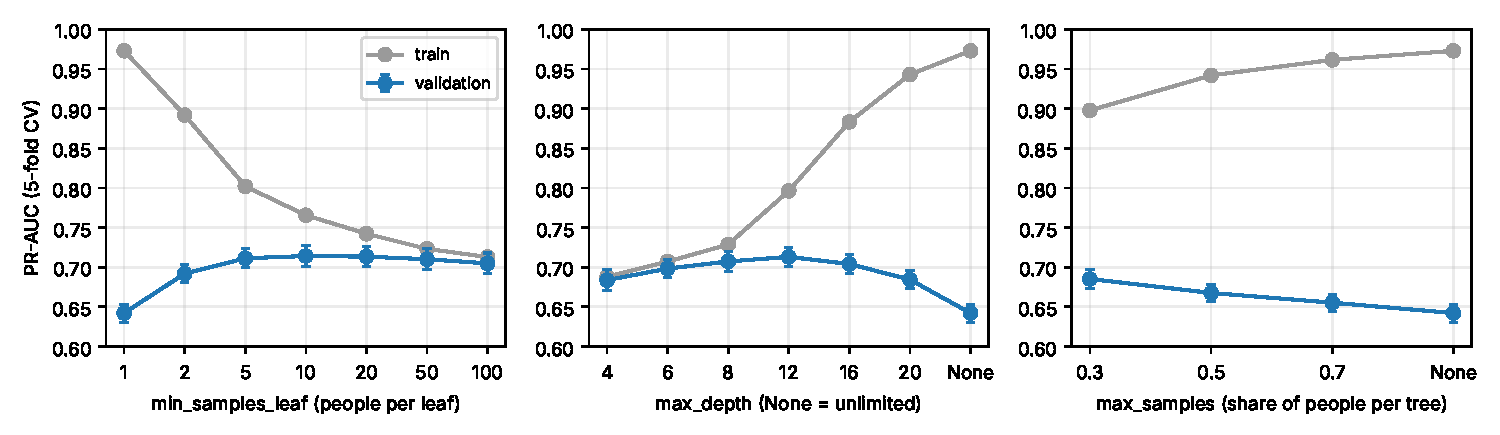
\includegraphics[width=\textwidth]{figures/rf_curves.pdf}
\caption{Random forest validation curves (5-fold CV, 200 trees, other settings at sklearn defaults; error bars = fold std). Left: the bias--variance picture, from memorizing (leaf 1) to underfitting (leaf 100). Centre: depth 4 underfits, unlimited depth overfits. Right: smaller samples per tree reduce overfitting.}
\label{fig:rf}
\end{figure}

\paragraph{Tuning v2 (random forest).} Each choice of the v2 search space comes from a curve: settings with no or a harmful effect are fixed (300 trees, Gini, no class weights); each searched range is a plateau plus a margin (leaf 5--30, depth 8--20, split 2--200, \code{max\_samples} 30--100\%, \code{max\_features} in \{sqrt, log2, 0.3\}). Objective, budget and seed are those of v1, so the only difference is the search space. A full grid over these settings would need thousands of combinations; Optuna's first 10 trials are random search, then its TPE sampler concentrates on promising regions (Session~5). All 25 trials scored between 0.709 and 0.715: the space lies on the plateau, and the guided trials added 0.0005 over the random ones. The settings interact: alone the best leaf size was 10, but with 39\% of people per tree Optuna prefers leaf 6.

\begin{table}[H]
\centering\small
\begin{tabular}{@{}lccccc@{}}
\toprule
Random forest & Train PR-AUC & Val.\ PR-AUC & Gap & Val.\ ROC-AUC & Val.\ Brier \\
\midrule
One tree, fully grown & 0.977 & 0.444 & 0.533 & 0.734 & 0.196 \\
sklearn defaults (100 trees, leaf 1) & 0.972 & 0.639 & 0.333 & 0.857 & 0.131 \\
Baseline (300 trees, leaf 5) & 0.803 & 0.711 & 0.092 & 0.890 & 0.111 \\
Tuned v1 (Optuna, 25 trials) & 0.749 & 0.715 & 0.035 & 0.891 & 0.136 \\
\textbf{Tuned v2} (space from the curves) & 0.754 & \textbf{0.715} & 0.039 & 0.891 & \textbf{0.110} \\
\bottomrule
\end{tabular}
\caption{Random forest, same 5 folds. v2 keeps v1's ranking with a small gap and trustworthy probabilities (best: leaf 6, depth 16, split 10, 39\% of people per tree, sqrt columns).}
\label{tab:rf}
\end{table}

\paragraph{Logistic regression.} Tuning v1 is the only tuning so far; no validation-curve diagnosis has been run for it \todo{Soumaya: logistic regression diagnosis / v2, if done}.

\paragraph{LightGBM.} \todo{Hadiqa: LightGBM diagnosis and tuning (\code{tuning/lightgbm.py}).}

\paragraph{Experiment tracking.} Every Optuna study is a parent MLflow run (model, version, budget, objective, CV scheme, best parameters and scores, optimization-history figure) with one nested run per trial (its hyperparameters, mean and standard deviation of PR-AUC and ROC-AUC, Brier score, per-fold metrics). Tuning v1 produced 78 runs (3 parents + 75 trials) and the random forest v2 26 more. Runs are stored in a local SQLite file; the best parameters of each version are versioned in Git (\code{tuning/results/<version>/}). \todo{MLflow screenshot, Appendix~\ref{app:mlflow}}

% ---------------------------------------------------------------
\section{Calibration}
\label{sec:calib}
\todo{reliability curve, Brier score and ECE of the final model; over- or under-confident; whether its probabilities can be trusted as-is}

\section{Explainability with SHAP}
\todo{global importance and local explanations of the final model; do the important features make business sense; proxy check by sex}

\section{Fairness and bias audit}
\label{sec:fair}
\todo{metrics by sex (selection rate, TPR, FPR, precision) against the definitions of Section 1; one mitigation; performance and fairness gaps before / after on the untouched test set}

\section{Final evaluation on the test set}
\label{sec:test}
\todo{final model, evaluated once on the 9{,}758 test people}

% ---------------------------------------------------------------
\section{Limitations and conclusion so far}

\begin{itemize}
\item \textbf{Data.} A 1994 US snapshot, with sex recorded as binary and an arbitrary \$50K threshold that limits its value as a fairness benchmark \cite{ding2021}. Results describe this population, not today's.
\item \textbf{Ceiling.} Six legitimate inputs carry about 0.71 PR-AUC of signal; we removed stronger but leaking or sex-revealing columns on purpose. More tuning does not raise this level; only new legitimate information could.
\item \textbf{Optimism.} Tuned scores are selected on the same folds they are scored on; the test evaluation will give the honest figure.
\end{itemize}

So far, the model is as good as the six inputs allow: three model families and two tunings of the random forest reach the same level, and the random forest's tuning v2 shows how a search space read from validation curves keeps that ranking with trustworthy probabilities. The EDA shows that the inputs are strong proxies for sex; the next stages test whether the model reproduces the income gap between women and men, and what reducing it costs. \todo{final conclusion}

% ---------------------------------------------------------------
\section*{Contribution statement}

\begin{table}[H]
\centering\small
\begin{tabularx}{\textwidth}{@{}lX@{}}
\toprule
Member & Contributions \\
\midrule
Manel Rahali & GitHub repository and branch workflow; EDA (data integrity, types, outliers, rare categories, features vs target, leakage audit, cleaning and split, preview of the transformed data); \code{src/data.py}; preprocessing in \code{src/pipeline.py}; project architecture (\code{src/} library, \code{tuning/} scripts); random forest diagnosis, validation curves and tuning v2; README; report coordination. \\
Soumaya Atoui & Business case and target orientation; feature engineering; EDA steps on groups, proxies and framing; baseline progression, Optuna tuning v1 and MLflow tracking; calibration and fairness scripts; findings log \todo{confirm}. \\
Hadiqa Javaid & LightGBM diagnosis and tuning \todo{complete}. \\
\bottomrule
\end{tabularx}
\end{table}

\paragraph{Use of AI coding assistants.} We used Claude (Anthropic) as an assistant: to discuss course concepts, to draft and refactor code (project architecture, diagnosis and tuning scripts), and to draft parts of this report from our findings log. Every script was run by the team, every number comes from our runs, and all methodological choices were reviewed by us. \todo{teammates: add your own use, if any}

\begin{thebibliography}{9}\small
\bibitem{kohavi1996} R.~Kohavi. Scaling up the accuracy of naive-Bayes classifiers: a decision-tree hybrid. \emph{KDD}, 1996 (the Adult dataset).
\bibitem{chakrabarty2018} N.~Chakrabarty, S.~Biswas. A statistical approach to adult census income level prediction. arXiv:1810.10076, 2018.
\bibitem{ding2021} F.~Ding, M.~Hardt, J.~Miller, L.~Schmidt. Retiring Adult: new datasets for fair machine learning. \emph{NeurIPS}, 2021.
\bibitem{hardt2016} M.~Hardt, E.~Price, N.~Srebro. Equality of opportunity in supervised learning. \emph{NeurIPS}, 2016.
\bibitem{ke2017} G.~Ke et al. LightGBM: a highly efficient gradient boosting decision tree. \emph{NeurIPS}, 2017.
\bibitem{akiba2019} T.~Akiba et al. Optuna: a next-generation hyperparameter optimization framework. \emph{KDD}, 2019.
\end{thebibliography}

% ---------------------------------------------------------------
\appendix
\section{Experiment tracking}
\label{app:mlflow}
\todo{screenshot of the MLflow runs table (parent run and its 25 trials) and the parallel-coordinates view of the random forest v2 trials}

\section{Reproducing the results}
From the project root, with the environment active: \code{python3 -m src.data}; \code{python3 -m src.pipeline}; \code{python3 -m tuning.baseline}; \code{python3 -m tuning.random\_forest baseline} and \code{curves}; \code{python3 -m tuning.tune --version v2 --model rf}. Setup and troubleshooting are in the README.

\end{document}
